\documentclass{article}
\usepackage[utf8]{inputenc}
\usepackage{tikz}
\usetikzlibrary{calc,shapes.multipart,chains,arrows}

\title{Data structures and Algorithms in java.}
\author{Author: Anyuru David Derrick }
\date{\today}

\begin{document}
\begin{titlepage}
    \maketitle
\end{titlepage}

\begin{center}
    \textbf{Task3}\\    
\end{center}

\begin{flushleft}
    \textbf{Question 1: } From the adjacency matrix, draw a graph.\\ 
    \textbf{Solution:} \\ 
    \underline{Graph}  
\end{flushleft}    

\begin{center}
    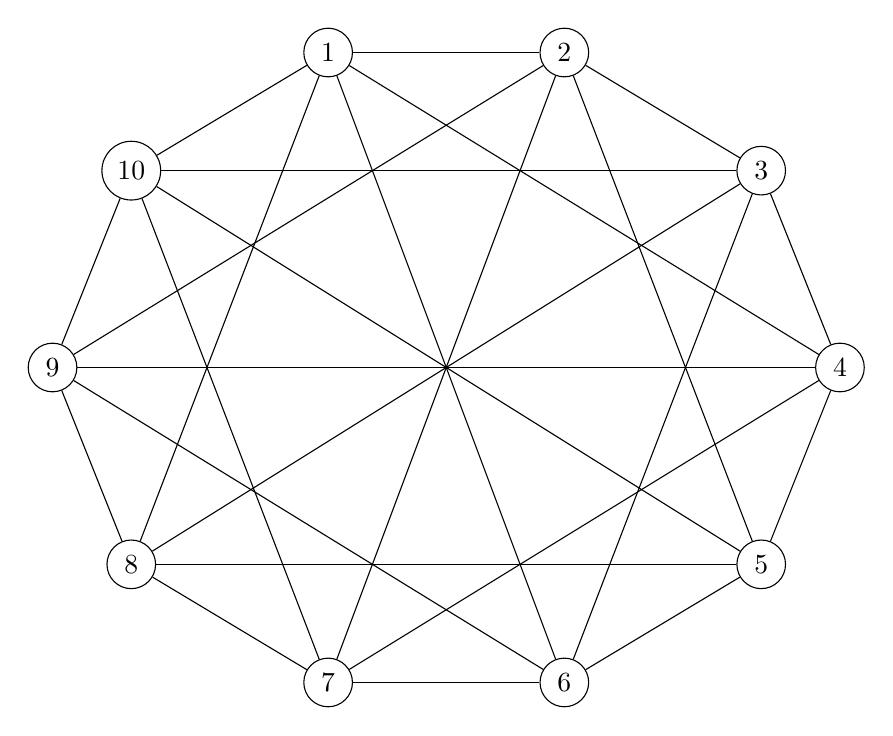
\begin{tikzpicture}[main/.style = {draw, circle}] 
    
    % Nodes
    \node[main] (1) at (5,12) {1};  
    \node[main] (2) at (8,12) {2};
    \node[main] (3) at (10.5,10.5) {3};
    \node[main] (4) at (11.5,8) {4};
    \node[main] (5) at (10.5,5.5) {5};
    \node[main] (6) at (8, 4) {6};
    \node[main] (7) at (5, 4) {7};
    \node[main] (8) at (2.5, 5.5) {8};
    \node[main] (9) at (1.5, 8) {9};
    \node[main] (10) at (2.5,10.5) {10};

    % Edges
    \draw (1) -- (2);
    \draw (1) -- (4);
    \draw (1) -- (6);
    \draw (1) -- (8);
    \draw (1) -- (10);
    \draw (2) -- (3);
    \draw (2) -- (5);
    \draw (2) -- (7);
    \draw (2) -- (9);
    \draw (3) -- (4);
    \draw (3) -- (6);
    \draw (3) -- (8);
    \draw (3) -- (10);
    \draw (4) -- (5);
    \draw (4) -- (7);
    \draw (4) -- (9);
    \draw (5) -- (6);
    \draw (5) -- (8);
    \draw (5) -- (10);
    \draw (6) -- (7);
    \draw (6) -- (9);
    \draw (7) -- (8);
    \draw (7) -- (10);
    \draw (8) -- (9);
    \draw (9) -- (10);
    
    \end{tikzpicture}

\end{center}
\begin{flushleft}
    \textbf{Question 2: } Construct an adjacency list and present it latex.\\ 
    \textbf{Solution:} \\ 
    \underline{Adjacency list}  
\end{flushleft}  

\begin{flushleft}
    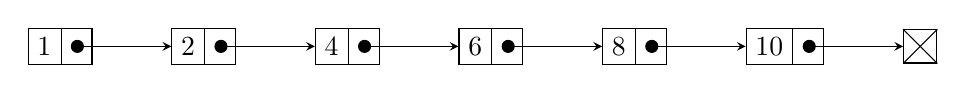
\begin{tikzpicture}[list/.style={rectangle split, rectangle split parts=2,
    draw, rectangle split horizontal}, >=stealth, start chain]
    \node[list,on chain] (X) {1};  
    \node[list,on chain] (A) {2};
    \node[list,on chain] (B) {4};
    \node[list,on chain] (C) {6};
    \node[list,on chain] (D) {8};
    \node[list,on chain] (E) {10};
    \node[on chain,draw,inner sep=6pt] (F) {};
    \draw (F.north east) -- (F.south west);
    \draw (F.north west) -- (F.south east);
    \draw[*->] let \p1 = (X.two), \p2 = (X.center) in (\x1,\y2) -- (A);
    \draw[*->] let \p1 = (A.two), \p2 = (A.center) in (\x1,\y2) -- (B);
    \draw[*->] let \p1 = (B.two), \p2 = (B.center) in (\x1,\y2) -- (C);
    \draw[*->] let \p1 = (C.two), \p2 = (C.center) in (\x1,\y2) -- (D);
    \draw[*->] let \p1 = (D.two), \p2 = (D.center) in (\x1,\y2) -- (E);
    \draw[*->] let \p1 = (E.two), \p2 = (E.center) in (\x1,\y2) -- (F);
    \end{tikzpicture}\\ 
    
    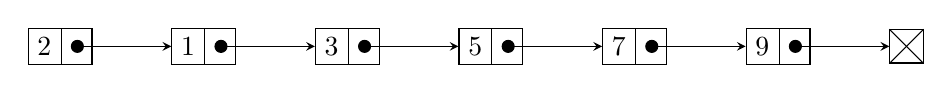
\begin{tikzpicture}[list/.style={rectangle split, rectangle split parts=2,
    draw, rectangle split horizontal}, >=stealth, start chain]
    \node[list,on chain] (X) {2};  
    \node[list,on chain] (A) {1};
    \node[list,on chain] (B) {3};
    \node[list,on chain] (C) {5};
    \node[list,on chain] (D) {7};
    \node[list,on chain] (E) {9};
    \node[on chain,draw,inner sep=6pt] (F) {};
    \draw (F.north east) -- (F.south west);
    \draw (F.north west) -- (F.south east);
    \draw[*->] let \p1 = (X.two), \p2 = (X.center) in (\x1,\y2) -- (A);
    \draw[*->] let \p1 = (A.two), \p2 = (A.center) in (\x1,\y2) -- (B);
    \draw[*->] let \p1 = (B.two), \p2 = (B.center) in (\x1,\y2) -- (C);
    \draw[*->] let \p1 = (C.two), \p2 = (C.center) in (\x1,\y2) -- (D);
    \draw[*->] let \p1 = (D.two), \p2 = (D.center) in (\x1,\y2) -- (E);
    \draw[*->] let \p1 = (E.two), \p2 = (E.center) in (\x1,\y2) -- (F);
\end{tikzpicture}\\

% 3
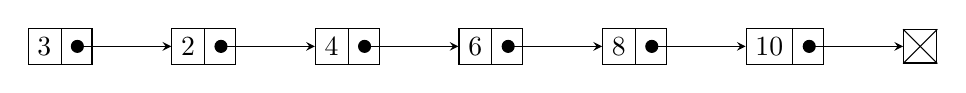
\begin{tikzpicture}[list/.style={rectangle split, rectangle split parts=2,
    draw, rectangle split horizontal}, >=stealth, start chain]
    \node[list,on chain] (X) {3};  
    \node[list,on chain] (A) {2};
    \node[list,on chain] (B) {4};
    \node[list,on chain] (C) {6};
    \node[list,on chain] (D) {8};
    \node[list,on chain] (E) {10};
    \node[on chain,draw,inner sep=6pt] (F) {};
    \draw (F.north east) -- (F.south west);
    \draw (F.north west) -- (F.south east);
    \draw[*->] let \p1 = (X.two), \p2 = (X.center) in (\x1,\y2) -- (A);
    \draw[*->] let \p1 = (A.two), \p2 = (A.center) in (\x1,\y2) -- (B);
    \draw[*->] let \p1 = (B.two), \p2 = (B.center) in (\x1,\y2) -- (C);
    \draw[*->] let \p1 = (C.two), \p2 = (C.center) in (\x1,\y2) -- (D);
    \draw[*->] let \p1 = (D.two), \p2 = (D.center) in (\x1,\y2) -- (E);
    \draw[*->] let \p1 = (E.two), \p2 = (E.center) in (\x1,\y2) -- (F);
\end{tikzpicture}\\

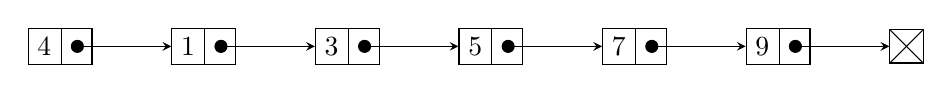
\begin{tikzpicture}[list/.style={rectangle split, rectangle split parts=2,
    draw, rectangle split horizontal}, >=stealth, start chain]
    \node[list,on chain] (X) {4};  
    \node[list,on chain] (A) {1};
    \node[list,on chain] (B) {3};
    \node[list,on chain] (C) {5};
    \node[list,on chain] (D) {7};
    \node[list,on chain] (E) {9};
    \node[on chain,draw,inner sep=6pt] (F) {};
    \draw (F.north east) -- (F.south west);
    \draw (F.north west) -- (F.south east);
    \draw[*->] let \p1 = (X.two), \p2 = (X.center) in (\x1,\y2) -- (A);
    \draw[*->] let \p1 = (A.two), \p2 = (A.center) in (\x1,\y2) -- (B);
    \draw[*->] let \p1 = (B.two), \p2 = (B.center) in (\x1,\y2) -- (C);
    \draw[*->] let \p1 = (C.two), \p2 = (C.center) in (\x1,\y2) -- (D);
    \draw[*->] let \p1 = (D.two), \p2 = (D.center) in (\x1,\y2) -- (E);
    \draw[*->] let \p1 = (E.two), \p2 = (E.center) in (\x1,\y2) -- (F);
\end{tikzpicture}\\

% 5
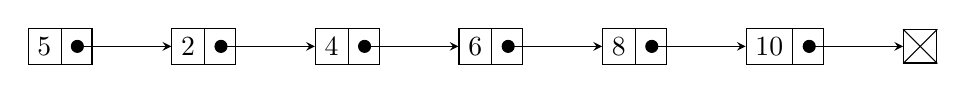
\begin{tikzpicture}[list/.style={rectangle split, rectangle split parts=2,
    draw, rectangle split horizontal}, >=stealth, start chain]
    \node[list,on chain] (X) {5};  
    \node[list,on chain] (A) {2};
    \node[list,on chain] (B) {4};
    \node[list,on chain] (C) {6};
    \node[list,on chain] (D) {8};
    \node[list,on chain] (E) {10};
    \node[on chain,draw,inner sep=6pt] (F) {};
    \draw (F.north east) -- (F.south west);
    \draw (F.north west) -- (F.south east);
    \draw[*->] let \p1 = (X.two), \p2 = (X.center) in (\x1,\y2) -- (A);
    \draw[*->] let \p1 = (A.two), \p2 = (A.center) in (\x1,\y2) -- (B);
    \draw[*->] let \p1 = (B.two), \p2 = (B.center) in (\x1,\y2) -- (C);
    \draw[*->] let \p1 = (C.two), \p2 = (C.center) in (\x1,\y2) -- (D);
    \draw[*->] let \p1 = (D.two), \p2 = (D.center) in (\x1,\y2) -- (E);
    \draw[*->] let \p1 = (E.two), \p2 = (E.center) in (\x1,\y2) -- (F);
    \end{tikzpicture}\\
    
    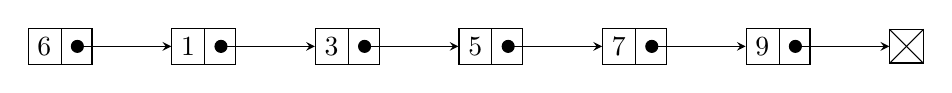
\begin{tikzpicture}[list/.style={rectangle split, rectangle split parts=2,
    draw, rectangle split horizontal}, >=stealth, start chain]
    \node[list,on chain] (X) {6};  
    \node[list,on chain] (A) {1};
    \node[list,on chain] (B) {3};
    \node[list,on chain] (C) {5};
    \node[list,on chain] (D) {7};
    \node[list,on chain] (E) {9};
    \node[on chain,draw,inner sep=6pt] (F) {};
    \draw (F.north east) -- (F.south west);
    \draw (F.north west) -- (F.south east);
    \draw[*->] let \p1 = (X.two), \p2 = (X.center) in (\x1,\y2) -- (A);
    \draw[*->] let \p1 = (A.two), \p2 = (A.center) in (\x1,\y2) -- (B);
    \draw[*->] let \p1 = (B.two), \p2 = (B.center) in (\x1,\y2) -- (C);
    \draw[*->] let \p1 = (C.two), \p2 = (C.center) in (\x1,\y2) -- (D);
    \draw[*->] let \p1 = (D.two), \p2 = (D.center) in (\x1,\y2) -- (E);
    \draw[*->] let \p1 = (E.two), \p2 = (E.center) in (\x1,\y2) -- (F);
\end{tikzpicture}\\
    
    % 7
    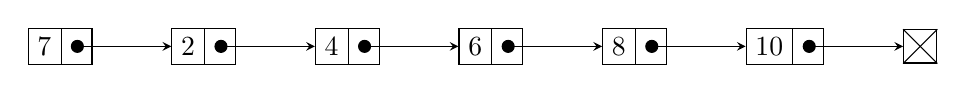
\begin{tikzpicture}[list/.style={rectangle split, rectangle split parts=2,
    draw, rectangle split horizontal}, >=stealth, start chain]
    \node[list,on chain] (X) {7};  
    \node[list,on chain] (A) {2};
    \node[list,on chain] (B) {4};
    \node[list,on chain] (C) {6};
    \node[list,on chain] (D) {8};
    \node[list,on chain] (E) {10};
    \node[on chain,draw,inner sep=6pt] (F) {};
    \draw (F.north east) -- (F.south west);
    \draw (F.north west) -- (F.south east);
    \draw[*->] let \p1 = (X.two), \p2 = (X.center) in (\x1,\y2) -- (A);
    \draw[*->] let \p1 = (A.two), \p2 = (A.center) in (\x1,\y2) -- (B);
    \draw[*->] let \p1 = (B.two), \p2 = (B.center) in (\x1,\y2) -- (C);
    \draw[*->] let \p1 = (C.two), \p2 = (C.center) in (\x1,\y2) -- (D);
    \draw[*->] let \p1 = (D.two), \p2 = (D.center) in (\x1,\y2) -- (E);
    \draw[*->] let \p1 = (E.two), \p2 = (E.center) in (\x1,\y2) -- (F);
    \end{tikzpicture}\\ 
    
    % 8
    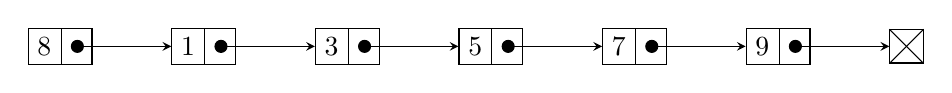
\begin{tikzpicture}[list/.style={rectangle split, rectangle split parts=2,
    draw, rectangle split horizontal}, >=stealth, start chain]
    \node[list,on chain] (X) {8};  
    \node[list,on chain] (A) {1};
    \node[list,on chain] (B) {3};
    \node[list,on chain] (C) {5};
    \node[list,on chain] (D) {7};
    \node[list,on chain] (E) {9};
    \node[on chain,draw,inner sep=6pt] (F) {};
    \draw (F.north east) -- (F.south west);
    \draw (F.north west) -- (F.south east);
    \draw[*->] let \p1 = (X.two), \p2 = (X.center) in (\x1,\y2) -- (A);
    \draw[*->] let \p1 = (A.two), \p2 = (A.center) in (\x1,\y2) -- (B);
    \draw[*->] let \p1 = (B.two), \p2 = (B.center) in (\x1,\y2) -- (C);
    \draw[*->] let \p1 = (C.two), \p2 = (C.center) in (\x1,\y2) -- (D);
    \draw[*->] let \p1 = (D.two), \p2 = (D.center) in (\x1,\y2) -- (E);
    \draw[*->] let \p1 = (E.two), \p2 = (E.center) in (\x1,\y2) -- (F);
\end{tikzpicture}\\
    
    % 9
    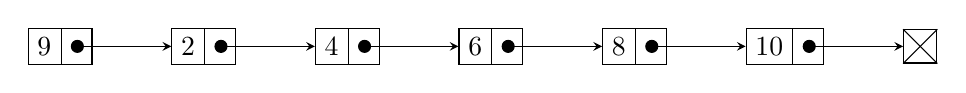
\begin{tikzpicture}[list/.style={rectangle split, rectangle split parts=2,
    draw, rectangle split horizontal}, >=stealth, start chain]
    \node[list,on chain] (X) {9};  
    \node[list,on chain] (A) {2};
    \node[list,on chain] (B) {4};
    \node[list,on chain] (C) {6};
    \node[list,on chain] (D) {8};
    \node[list,on chain] (E) {10};
    \node[on chain,draw,inner sep=6pt] (F) {};
    \draw (F.north east) -- (F.south west);
    \draw (F.north west) -- (F.south east);
    \draw[*->] let \p1 = (X.two), \p2 = (X.center) in (\x1,\y2) -- (A);
    \draw[*->] let \p1 = (A.two), \p2 = (A.center) in (\x1,\y2) -- (B);
    \draw[*->] let \p1 = (B.two), \p2 = (B.center) in (\x1,\y2) -- (C);
    \draw[*->] let \p1 = (C.two), \p2 = (C.center) in (\x1,\y2) -- (D);
    \draw[*->] let \p1 = (D.two), \p2 = (D.center) in (\x1,\y2) -- (E);
    \draw[*->] let \p1 = (E.two), \p2 = (E.center) in (\x1,\y2) -- (F);
    \end{tikzpicture}\\ 
    
    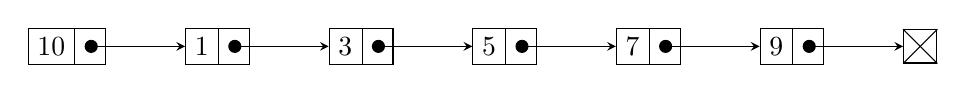
\begin{tikzpicture}[list/.style={rectangle split, rectangle split parts=2,
    draw, rectangle split horizontal}, >=stealth, start chain]
    \node[list,on chain] (X) {10};  
    \node[list,on chain] (A) {1};
    \node[list,on chain] (B) {3};
    \node[list,on chain] (C) {5};
    \node[list,on chain] (D) {7};
    \node[list,on chain] (E) {9};
    \node[on chain,draw,inner sep=6pt] (F) {};
    \draw (F.north east) -- (F.south west);
    \draw (F.north west) -- (F.south east);
    \draw[*->] let \p1 = (X.two), \p2 = (X.center) in (\x1,\y2) -- (A);
    \draw[*->] let \p1 = (A.two), \p2 = (A.center) in (\x1,\y2) -- (B);
    \draw[*->] let \p1 = (B.two), \p2 = (B.center) in (\x1,\y2) -- (C);
    \draw[*->] let \p1 = (C.two), \p2 = (C.center) in (\x1,\y2) -- (D);
    \draw[*->] let \p1 = (D.two), \p2 = (D.center) in (\x1,\y2) -- (E);
    \draw[*->] let \p1 = (E.two), \p2 = (E.center) in (\x1,\y2) -- (F);
\end{tikzpicture}\\
\end{flushleft}
\end{document}
